% 单摆
\pentry{简谐振子\upref{SHO}, 匀速圆周运动\upref{CMAD}}

理想的单摆由一个质点和一个质量不计的细绳(或细杆)组成. 绳的一头连接质点, 另一头固定不动. 我们来对单摆做受力分析. 如\autoref{Pend_fig1}, 令质点质量为 $m$, 受重力大小为 $mg$, 受绳的拉力大小为 $T$. 将重力沿与绳平行的方向和垂直的方向正交分解, 分力大小分别为 $mg\cos\theta$ 和 $mg\sin\theta$. 由于绳的限制, 质点只允许做圆周运动, 所以绳的拉力与重力平行绳的分量必然提供质点的向心力.
\begin{equation}
T - mg\cos\theta = ma_c
\end{equation}
对于变速圆周运动, 向心加速度仍然可以用 $a_c = v^2/L$ 求解, 其中 $L$ 是绳长即圆的半径(证明见 “变速圆周运动”).%未完成
在求单摆运动时, 拉力 $T$ 的大小并不重要, 我们更关心的是摆角 $\theta$ 随时间的变化.
\begin{figure}[ht]
\centering
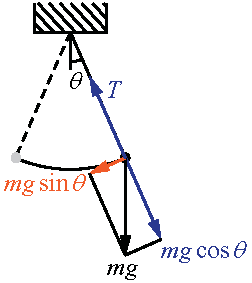
\includegraphics[width=4.5cm]{./figures/Pend.pdf}
\caption{单摆} \label{Pend_fig1}
\end{figure}

令质点向右运动时速度为正, 角速度和速度的关系为 $\dot\theta = v/L$, 对其两边求导得角加速度和加速度的关系
\begin{equation}
\ddot\theta = a_\theta/L
\end{equation}
其中 $a_\theta$ 是质点延垂直绳方向的加速度. 现在沿垂直绳方向运用牛顿第二定律, 并代入上式中的 $a_\theta$ 得
\begin{equation}
-mg\sin\theta = ma_\theta = -m\ddot\theta L
\end{equation}
两边消去质量可得摆角 $\theta$ 关于时间的二阶微分方程.
\begin{equation}\label{Pend_eq4}
L\ddot\theta = - g\sin\theta
\end{equation}
解出该方程即可得到单摆做任意幅度摆动的规律. 虽然我们还不知道方程的解, 但观察方程可知单摆的运动规律只与摆长 $L$ 和重力加速度 $g$ 有关, 而与质点的质量无关. 所以改变同一单摆的质量不会改变它的运动规律.

\subsection{小幅度摆动}
\pentry{小角正弦值极限\upref{LimArc}}

遗憾的是, \autoref{Pend_eq4} 的解并不能用有限个基本初等函数表示. 我们先来考虑一种简单的情况, 即单摆进行小的幅度摆动. 当 $\theta \to 0$ 时, 我们可以把\autoref{Pend_eq4} 中的 $\sin\theta$ 近似为 $\theta$. 令质点从最低点到当前位置之间的弧长为 $s$, 则有 $s = \theta L$ 和 $\ddot s = a_\theta = \ddot\theta L$, \autoref{Pend_eq4} 变为 $s$ 的微分方程
\begin{equation}
\ddot s = - \frac gL s
\end{equation}
观察该式可以发现其结构与简谐振子的微分方程(\autoref{SHO_eq1}\upref{SHO}) 非常相似. 用同样的方法, 可得通解为
\begin{equation}
s = A\cos(\omega t + \varphi _0)  \qquad \qty(\omega  = \sqrt {g/L})
\end{equation}
考虑到 $\theta \to 0$ 的情况下, 圆弧可以近似为线段, 所以可以认为此时质点在做一维简谐运动, 用坐标 $x$ 代替弧长 $s$.



